\section{Introduction}
The noise pollution is one of the main issue of the XXI\textsuperscript{ème} century. It causes usual annoyance but it's also threat health. The European Union highlights the risks of noise pollution \cite{Noise_in_Europe}. The transports cause the high noise pollution.  A considerable effort has be made to reduce the emissions and continues to be made.\\ 
In the aircraft field, the noise has to be reduced inside to keep a relative comfort for the passengers and also outside in the case because aircraft fly over habitations. The main source of noise in the aircraft is the engines.\\
The emission of noise in an engine is complex and due to different phenomenons. Nowadays, the usual engines type is by-pass turbofan engine. At the input of the duct, there is the admission of low pressure air. A fan push the air into the higher levels, the interaction between this fan and the stator is one of the principal source of noise. Thus, a high air ratio pass trough the by-pass duct. The second path is the principal duct. The combustion it's also a high source of emission. The air is ejection is called a jet flow. The interaction between the different flows velocity as the instationary flows are a source of noise. The following figure shows the different sources of noise in a by-pass turbofan engine.
\begin{figure}[H] \centering
    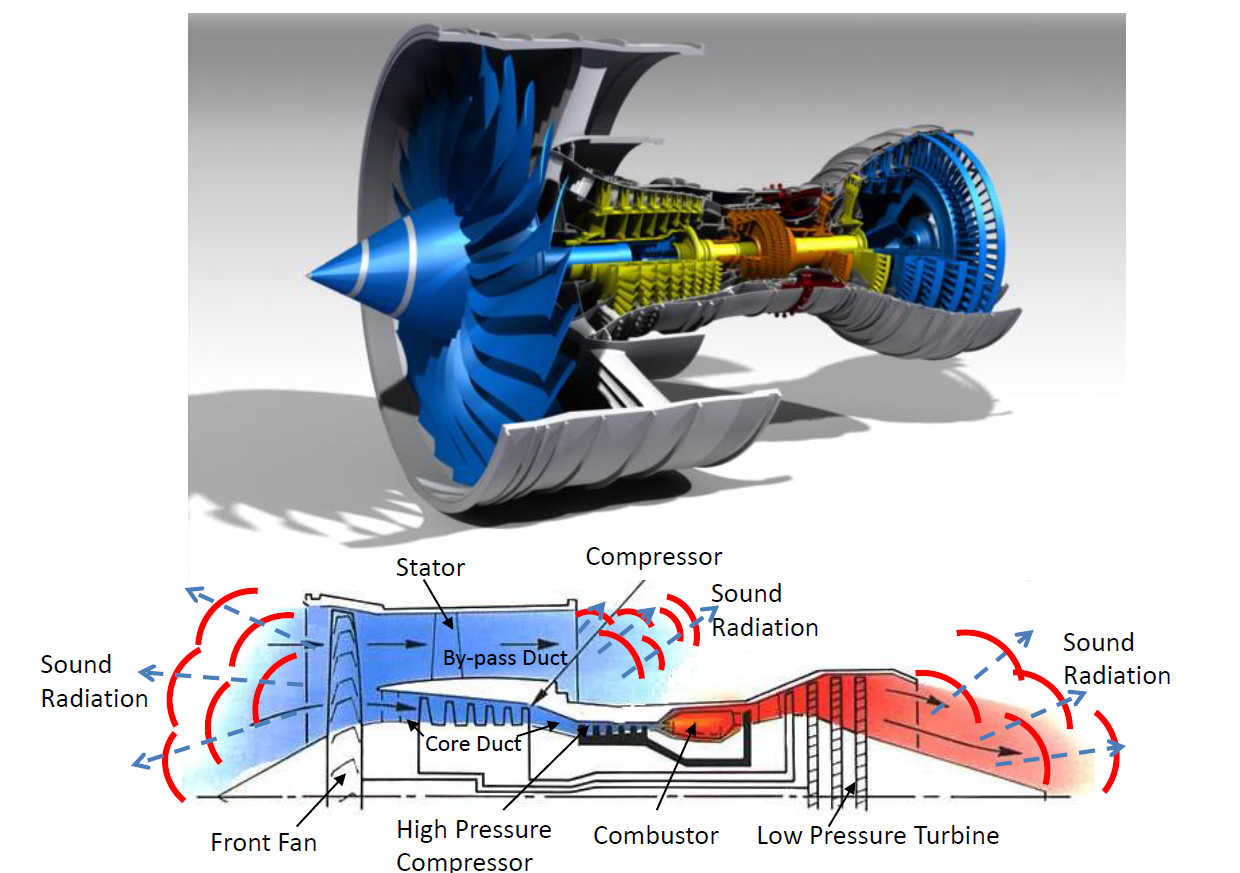
\includegraphics[scale=0.5]{Sources_in_engines}
    \caption{Different acoustic sources in engines \cite{Zhou_thesis}}
\end{figure}
To reduce the noise transmission, a liner acoustic is added in the engines walls. It is a perforated panel which contained a honeycomb structure. The small cavities can be compare to small Helmholtz resonators. The air in the orifices plays the role of mass and the cavity formed by the honeycomb structures acts as a spring.
\begin{figure}[H] \centering
\label{fig:Sources_in_engines2}
    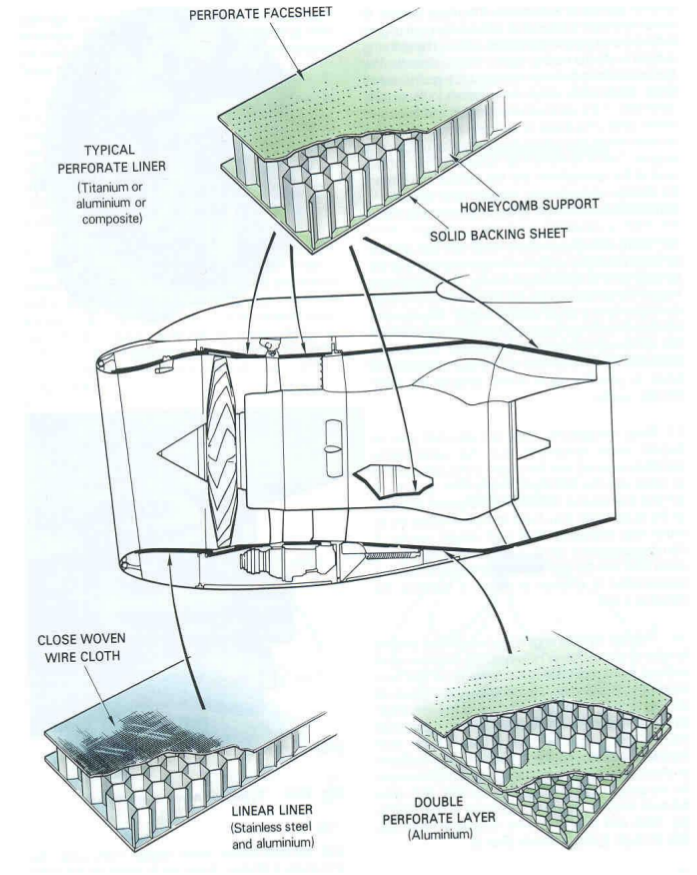
\includegraphics[scale=0.4]{typical_perforate_liner}
    \caption{Typical perforate liner \cite{The_jet_engine}}
\end{figure}
Aircraft suppliers need to well understand how work these liners to optimize the geometry or to add some porous material inside the honeycomb structures. However the problem is very difficult. Indeed the size of the acoustic waves in the engines are very higher than the size of the whole ($\sim$ 0.5mm). That's why it's very difficult to implement a finite-elements method. Some models are to be found to reduce this difficulty. The usually solution is to used the acoustic impedance of the liner:
\begin{itemize}
    \item First, the wall impedance is find with the acoustic theory applied to small cavities.
    \item The impedance of the liner is used in a macro model.
\end{itemize}
This master thesis is part of the IMAGE project (Innovative Methodologies and technologies for reducing Aircraft noise Generation and Emission) which is in collaboration with European and Chinese laboratories.
\clearpage